\Article{11}
Wenden wir uns nun unserem eigentlichen Gegenstand näher zu. Sind für den Modul $m=a+bi$ die Zahlen $f,f',f''$ usw. so beschaffen, dass sie erstens alle modulo $m$ paarweise inkongruent sind und zweitens jede ganze Zahl notwendig einer von ihnen kongruent sein muss, so nennen wir die
\SourceLeaf{326}
Gesamtheit der Zahlen $f,f',f''$ usw. das System der Primitivreste von $m$. Ihre Anzahl ist stets $=aa+bb$.

\Article{12}
Das System der Primitivreste kann auf viele Arten gebildet werden. Am einfachsten wählt man die Punkte innerhalb des Quadrats $0,m,(1+i)m,im$; hinzuzufügen sind jedoch noch
\begin{enumerate}
\item[I.] der Punkt oder die Größe $0$;
\item[II.] alle Punkte auf zwei einander nicht gegenüberliegenden Grenzlinien.
\end{enumerate}
Statt auf einer der $4$ Grenzlinien alle Punkte zu nehmen, kann man sie auch auf mehreren zugleich nehmen.

Die Auswahl dieser Punkte auf den Grenzlinien, falls dort welche liegen, kann auf mehrere Arten geschehen, die den obigen Bedingungen genügen. Die einfachste ist die folgende.

Man nehme auf der Grenzlinie $0,m$ alle Punkte zwischen $0$ und $\frac12m$, inklusive, und auf der Grenzlinie $0,im$ alle Punkte von $\frac12im$ bis $im$, exklusive, und verfahre bei den beiden anderen ähnlich.

Diese beiden Verfahren lassen sich so veranschaulichen:
\begin{center}\resizebox{.85\textwidth}{!}{\begin{tikzpicture}[x=1bp,y=-1bp,line cap=round,line join=round]
\path[use as bounding box] (0,0) rectangle (1230,440);
\begin{pgfinterruptboundingbox}
\draw[line width=2.2bp] (228,69) -- (72,214) -- (218,366) -- (373,219) -- (326,168);
\draw[line width=2.2bp] (322,163) -- (257,96);
\draw[line width=2.2bp] (250,90) -- (228,69);
\draw[line width=2bp] (148,136) circle[radius=5bp];
\draw[line width=2bp] (304,140) circle[radius=5bp];
\draw[line width=2bp] (297,284) circle[radius=5bp];
\draw[line width=2bp] (152,290) circle[radius=5bp];
\node[inner sep=0pt,outer sep=0pt,anchor=center] at (53,214) {\scalebox{3.5}{\ensuremath{m}}};
\node[inner sep=0pt,outer sep=0pt,anchor=center] at (228,48) {\scalebox{3.5}{\ensuremath{(1+i)m}}};
\node[inner sep=0pt,outer sep=0pt,anchor=center] at (399,220) {\scalebox{3.5}{\ensuremath{im}}};
\node[inner sep=0pt,outer sep=0pt,anchor=center] at (213,387) {\scalebox{3.5}{\ensuremath{0}}};
\draw[line width=2.2bp] (839,229) -- (993,77) -- (1143,234) -- (987,378) -- cycle;
\draw[line width=2bp] (878,197) circle[radius=5bp];
\draw[line width=2bp] (906,155) circle[radius=5bp];
\draw[line width=2bp] (951,112) circle[radius=5bp];
\draw[line width=2bp] (1023,116) circle[radius=5bp];
\draw[line width=2bp] (1069,151) circle[radius=5bp];
\draw[line width=2bp] (1112,193) circle[radius=5bp];
\draw[line width=2bp] (869,270) circle[radius=5bp];
\draw[line width=2bp] (915,303) circle[radius=5bp];
\draw[line width=2bp] (956,344) circle[radius=5bp];
\draw[line width=2bp] (984,373) circle[radius=5bp];
\draw[line width=2bp] (1024,352) circle[radius=5bp];
\draw[line width=2bp] (1055,309) circle[radius=5bp];
\draw[line width=2bp] (1098,269) circle[radius=5bp];
\node[inner sep=0pt,outer sep=0pt,anchor=center] at (819,229) {\scalebox{3.5}{\ensuremath{m}}};
\node[inner sep=0pt,outer sep=0pt,anchor=center] at (991,54) {\scalebox{3.5}{\ensuremath{(1+i)m}}};
\node[inner sep=0pt,outer sep=0pt,anchor=center] at (1166,236) {\scalebox{3.5}{\ensuremath{im}}};
\node[inner sep=0pt,outer sep=0pt,anchor=center] at (978,397) {\scalebox{3.5}{\ensuremath{0}}};
\end{pgfinterruptboundingbox}
\end{tikzpicture}
}\end{center}

\Article{13}
Schließt man von den Primitivpunkten aus:
\begin{enumerate}
\item[I.] nur den Punkt $0$, wenn $a$ gerade und $b$ ungerade ist, oder umgekehrt;
\item[II.] die Punkte $0$ und $\frac12(1+i)m$, wenn $a$ und $b$ beide ungerade sind;
\item[III.] die vier Punkte $0,\frac12m,\frac12(1+i)m,\frac12im$, wenn $a$ und $b$ beide gerade sind,
\end{enumerate}
so nennen wir die verbleibenden eigentliche Primitivpunkte und die ausgeschlossenen uneigentliche. Die Anzahl der ersteren ist also
\[
\begin{array}{rrcl}
\text{im Fall}&\mathrm{I}&=&aa+bb-1\\
&\mathrm{II}&=&aa+bb-2\\
&\mathrm{III}&=&aa+bb-4
\end{array}
\]
und damit stets durch $4$ teilbar.

\SourceLeaf{327}
\Article{14}
Diese eigentlichen Primitivpunkte lassen sich in $4$ Klassen $F,F',F'',F'''$ aufteilen, sodass
\[
\begin{array}{llll}
iF\equiv F'&iF'\equiv F''&iF''\equiv F'''&iF'''\equiv F\\
-F\equiv F''&-F'\equiv F'''&-F''\equiv F&-F'''\equiv F'\\
-iF\equiv F'''&-iF'\equiv F&-iF''\equiv F'&-iF'''\equiv F''
\end{array}
\]
\Needspace{17\baselineskip}
Dabei gilt nun der folgende äußerst wichtige Satz.

Es sei $M$ eine Zahl, die mit $m$ keinen Faktor gemeinsam hat. Von den Zahlen $MF$ gehören zur Klasse $F$ eine Anzahl von $n$,
\[
\begin{array}{cc}F'&n'\\F''&n''\\F'''&n'''\end{array}
\]
und der kleinste Rest von $n'+2n''+3n''$ modulo $4$ sei $=N$, also $N$ gleich einer der $4$ Zahlen $0,1,2,3$. Unter dieser Voraussetzung ist $N$ \emph{unabhängig} von der Aufteilung der Primitivreste in Klassen. Wir nennen ihn den Dezidenten des biquadratischen Verhältnisses der Zahl $M$ zu $m$.

\Article{15}
Die einfachste Art der Aufteilung ist allerdings die folgende:
\begin{center}\resizebox{.35\textwidth}{!}{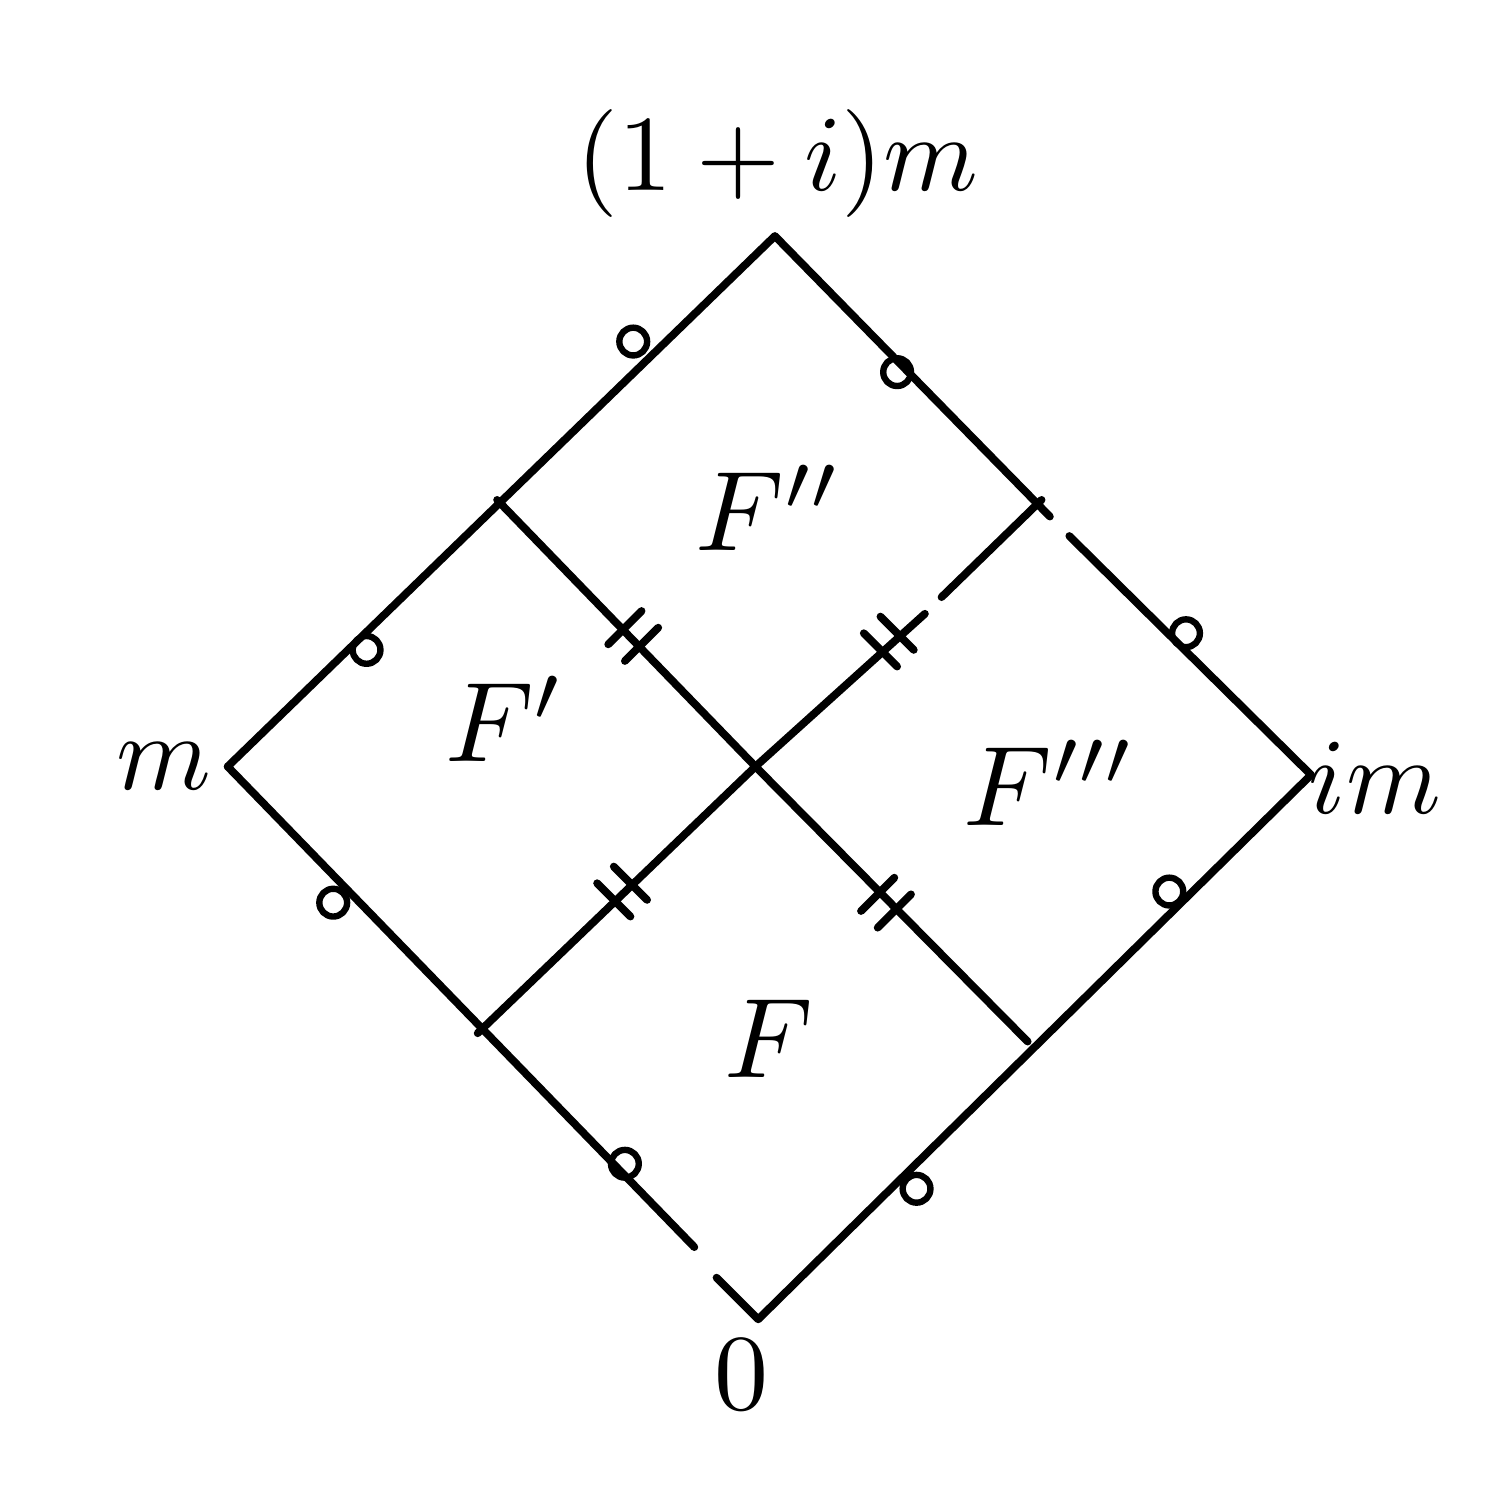
\begin{tikzpicture}[x=1bp,y=-1bp,line cap=round,line join=round]
\path[use as bounding box] (0,0) rectangle (520,520);
\begin{pgfinterruptboundingbox}
\draw[line width=2.8bp] (72,266) -- (269,75) -- (368,176);
\draw[line width=2.8bp] (375,183) -- (462,269) -- (263,465) -- (248,450);
\draw[line width=2.8bp] (240,439) -- (72,266);
\draw[line width=2.8bp] (169,170) -- (262,266) -- (360,365);
\draw[line width=2.8bp] (365,170) -- (329,205);
\draw[line width=2.8bp] (323,211) -- (262,266) -- (162,362);
\draw[line width=2.3bp] (218,113) circle[radius=5bp];
\draw[line width=2.3bp] (313,124) circle[radius=5bp];
\draw[line width=2.3bp] (122,224) circle[radius=5bp];
\draw[line width=2.3bp] (417,218) circle[radius=5bp];
\draw[line width=2.3bp] (110,315) circle[radius=5bp];
\draw[line width=2.3bp] (411,311) circle[radius=5bp];
\draw[line width=2.3bp] (215,409) circle[radius=5bp];
\draw[line width=2.3bp] (320,418) circle[radius=5bp];
\draw[line width=2.8bp] (209,222) -- (221,210);
\draw[line width=2.8bp] (215,228) -- (227,216);
\draw[line width=2.8bp] (301,218) -- (313,230);
\draw[line width=2.8bp] (307,212) -- (319,224);
\draw[line width=2.8bp] (205,308) -- (217,320);
\draw[line width=2.8bp] (211,302) -- (223,314);
\draw[line width=2.8bp] (300,318) -- (312,306);
\draw[line width=2.8bp] (306,324) -- (318,312);
\node[inner sep=0pt,outer sep=0pt,anchor=center] at (267,173) {\scalebox{4.1}{\ensuremath{F''}}};
\node[inner sep=0pt,outer sep=0pt,anchor=center] at (172,249) {\scalebox{4.1}{\ensuremath{F'}}};
\node[inner sep=0pt,outer sep=0pt,anchor=center] at (368,272) {\scalebox{4.1}{\ensuremath{F'''}}};
\node[inner sep=0pt,outer sep=0pt,anchor=center] at (267,364) {\scalebox{4.1}{\ensuremath{F}}};
\node[inner sep=0pt,outer sep=0pt,anchor=center] at (49,266) {\scalebox{3.9}{\ensuremath{m}}};
\node[inner sep=0pt,outer sep=0pt,anchor=center] at (270,49) {\scalebox{3.9}{\ensuremath{(1+i)m}}};
\node[inner sep=0pt,outer sep=0pt,anchor=center] at (485,270) {\scalebox{3.9}{\ensuremath{im}}};
\node[inner sep=0pt,outer sep=0pt,anchor=center] at (257,485) {\scalebox{3.9}{\ensuremath{0}}};
\end{pgfinterruptboundingbox}
\end{tikzpicture}
}\end{center}
In besonderen Fällen kann jedoch eine andere Aufteilung vorteilhafter sein.

\Article{16}
Sind $f,f',f''$ usw. sämtliche Primitivreste des Moduls $m$, so gilt
\SourceLeaf{328}
\[
\begin{aligned}
&S(z+\tfrac fm,\ z'+\tfrac fm,\ z''+\tfrac fm,\ \text{usw.})\\
&+S(z+\tfrac{f'}m,\ z'+\tfrac{f'}m,\ z''+\tfrac{f'}m,\ \text{usw.})\\
&+S(z+\tfrac{f''}m,\ z'+\tfrac{f''}m,\ z''+\tfrac{f''}m,\ \text{usw.})\\
&+\text{usw.}\\
&=S(mz,mz',mz'',\ \text{usw.}
\end{aligned}
\]
